\documentclass{article}       %On doit définir la classe de document (
\usepackage[utf8]{inputenc}  %Pour écrire de base (doit tjrs être là)
\usepackage{supertabular} %Si jamais des tableaux vont sur plus qu'une page
\usepackage[T1]{fontenc}  %Pour faire des ë,ö,û,...
\usepackage{icomma}       %Pour écrire 1,8 au lieu de 1, 8 (espace après la virgule en mode math)

\usepackage{array}     %Pour pouvoir faire des matrices et tableaux
\usepackage{color}     %Pour écrire du texte en couleur
\usepackage{amsmath,mathtools}   %Pour écrire des équations
\usepackage{amssymb,amsfonts}   %Pour loader des variables, lettres, flèches, signes...
\usepackage{esint}     %Pour faire des intégrales fermées et doubles
\usepackage{multirow}  %Pour fusionner des cases dans un tableau
\usepackage{float}     %Pour les figures flottantes et placer les figures dans le texte
\usepackage{graphicx}  %Pour intégrer des graphiques, images et photos..
\usepackage{tikz}   %dessiner toute sorte de belles choses.. Pratiquement sans fin ;)
\usepackage[left=2.5cm,right=2.5cm,top=3cm,bottom=3cm]{geometry} %Pour controler les marges
\usepackage{booktabs}
\usepackage{hyperref}  %Pour mettre des liens de références dans le texte
\usepackage[francais]{babel}  %Le dictionnaire français et permet aussi de comprendre les lettres françaises
\usepackage{caption}   %Pour pouvoir mettre des légendes aux figures «captions»
\captionsetup[table]{name = Tableau}
\usepackage{subcaption}
\usepackage{gensymb} %Pour avoir des symboles
\usepackage{tabulary}  %Pour faire des tableaux
\usepackage{fancyhdr}  %Pour définir des en-têtes et pieds de page fancy 
\usepackage{siunitx}   %Pour écrire des unités du système international
\usepackage{textcomp} 
\usepackage[siunitx]{circuitikz}  %dessiner des circuits électroniques

\usepackage{afterpage}

\newcommand\blankpage{%
    \null
    \thispagestyle{empty}%
    \addtocounter{page}{-1}%
    \newpage}
    
\newcommand{\HRule}{\rule{\linewidth}{0.5mm}}

\usepackage{parskip}         %Pour gérer les alinéas et les espaces entre les paragraphes
\setlength{\parindent}{0pt}  %Alinéas
\setlength{\parskip}{15pt}  %Espace entre paragraphes

\setlength\extrarowheight{2pt}



\usepackage{fancyhdr}
\pagestyle{fancy}
\usepackage{lastpage}
\renewcommand\headrulewidth{1pt}
\fancyhead[L]{\textbf{Statistiques des speckles}}
\fancyhead[C]{}
\fancyhead[R]{Quentin Perry-Auger}
\renewcommand\footrulewidth{1pt}
\fancyfoot[C]{\textbf{Page \thepage}}
%\fancyfoot[R]{Jeudi $1^{er}$ Décembre 2016}


\newfloat{Graphique}{tbp}{lop}

\def\changemargin#1#2{\list{}{\rightmargin#2\leftmargin#1}\item[]}
\let\endchangemargin=\endlist 

\usepackage{listingsutf8}
\usepackage{listings}
\definecolor{codegreen}{rgb}{0,0.6,0}
\definecolor{codegray}{rgb}{0.5,0.5,0.5}
\definecolor{codepurple}{rgb}{0.58,0,0.82}
\definecolor{backcolour}{rgb}{0.95,0.95,0.92}

\lstset{inputencoding=utf8/latin1}
\lstdefinestyle{mystyle}{
    backgroundcolor=\color{backcolour},   
    commentstyle=\color{codegreen},
    keywordstyle=\color{magenta},
    numberstyle=\tiny\color{codegray},
    stringstyle=\color{codepurple},
    basicstyle=\footnotesize,
    breakatwhitespace=false,         
    breaklines=true,                 
    captionpos=b,                    
    keepspaces=true,                 
    numbers=left,                    
    numbersep=5pt,                  
    showspaces=false,                
    showstringspaces=false,
    showtabs=false,                  
    tabsize=2
}
\lstset{style=mystyle}

\usepackage[stable]{footmisc}
%\usepackage[bottom]{footmisc}


\begin{document}   %On commence TOUUUUUJOURS avec \begin{document} [....]  \end{document}

\begin{titlepage}  %Faire une page titre qui ne sera pas comptée, ni paginée
\begin{center}   %Pour centrer tout ce qu'il y a entre \begin et \end 

\includegraphics[scale=0.5]{fig/logo.png}\\
\vspace{1cm}


\HRule\\[0.4cm]
{\large\bfseries Microscope HiLo pour imagerie calcique des poissons zèbre}
\HRule\\[1.75cm]


\vfill

{\bfseries Quentin Perry-Auger (\url{quentin.perry-auger.1@ulaval.ca})}

\vfill

Stagiaire CERVO\\ Été 2018


\vfill

\end{center}

\textbf{\Large Résumé}

Ce rapport présente le processus d'assemblage et le fonctionnement du microscope HiLo pour zebrafish tel qu'il est à date du 25 août 2018. Dans les prochaines sections, la méthode HiLo sera d'abord détaillée, de même que chaque partie de la structure du microscope. Enfin, un bref compte-rendu accompagné de quelques résultats sera présenté afin de donner des lignes directrices sur ce qu'il reste à faire et ainsi d'avoir une idée d'où le projet se dirige. 

\end{titlepage}



\section{La microscopie HiLo}

La microscopie HiLo est une méthode de microscopie à fluorescence grand champ, c'est-à-dire que tout l'échantillon est illuminé et, ainsi, la fluorescence captée ne provient pas uniquement du plan focal \cite{Mertz2008}. Toutefois, un sectionnement optique peut être obtenu par traitement mathématique post-acquisition. Afin d'effectuer ce sectionnement, deux images sont nécessaires: une image avec illumination uniforme et une image avec speckles (tavelures)\footnote{Le terme francophone pour des speckles est tavelures, mais ils seront appelés speckles dans cet ouvrage puisque ce phénomène est mieux connu sous ce nom \cite{Wiki}}. Les speckles sont une forme de granularité qui émerge de l'interférence d'un grand nombre de phaseurs aléatoires. Les speckles sont dit complètement développés si la fonction de densité de probabilité de l'intensité a une forme exponentielle décroissante \cite{Manuel}.

Le principe de la technique HiLo est de reconstruire l'image au plan focal en sommant deux images, soient une avec seulement des hautes fréquences spatiales et une avec seulement des basses fréquences spatiales (la fréquence de coupure étant la même pour les deux images). Le traitement HiLo permet donc de passer de deux images brutes (uniforme et speckles) à deux images traitées (hautes fréquences et basses fréquences), puis finalement à l'image HiLo en sommant ces dernières. Le résultat final est une image avec sectionnement optique et dont l'intensité est proportionnelle à la concentration de fluorophores \cite{Mertz2008}.

\subsection{Image Hi (hautes fréquences)}
\label{ImagesHi}

Obtenir les hautes fréquences présentes au plan focal est la partie simple du traitement HiLo. Puisqu'un microscope à fluorescence à illumination uniforme effectue intrinsèquement un sectionnement optique pour les fréquences spatiales non nulles \cite{Mertz2008}, il suffit de filtrer l'image uniforme avec un filtre passe-haut. Le filtre passe-haut HP est défini de sorte que \cite{Mertz2008}

\begin{equation*}
    \text{HP}(\kappa_{c}) = \frac{1}{2} 
\end{equation*},

où $\kappa_{c}$ est la fréquence de coupure du filtre.

\subsection{Image Lo (basses fréquences)}
\label{ImagesLo}

Puisqu'un microscope à illumination uniforme ne performe pas de sectionnement optique pour la fréquence spatiale nulle, il est impossible de récupérer les basses fréquences spatiales seulement au plan focal en appliquant un filtre. C'est ici que l'illumination avec speckles entre en jeu. On utilise le fait que le contraste des speckles complètement développés est de 1 au plan focal et tend vers 0 avec le défocus. Ainsi, le contraste est un indicateur de la quantité de lumière qui provient du plan focal \cite{Mertz2008}.

Afin d'avoir un microscope HiLo rapide et efficace, l'illumination uniforme est obtenue à partir de l'illumination avec speckles. Pour ce faire, on fait bouger rapidement et de façon aléatoire les speckles de façon à ce que leur mouvement soit beaucoup plus rapide que le temps d'acquisition de la caméra. Ainsi, l'illumination paraît uniforme sur les images et l'intensité obtenue est la moyenne de l'intensité des speckles. Les images prises avec illumination uniforme et avec speckles peuvent être écrite sous la forme des équations suivantes, respectivement \cite{Mertz2011}:

\begin{equation*}
    I_{u} = \int \int \text{PSF}_{det}(\vec{\rho_{d}} - \vec{\rho}, z)\text{O}(\vec{\rho}, z)<\text{S}>\text{d}^{2}\vec{\rho}\text{d}z
\end{equation*}

\begin{equation*}
    I_{s} = \int \int \text{PSF}_{det}(\vec{\rho_{d}} - \vec{\rho}, z)\text{O}(\vec{\rho}, z)\text{S}(\vec{\rho}, z)\text{d}^{2}\vec{\rho}\text{d}z
\end{equation*}

où $\text{PSF}_{det}(\vec{\rho}, z)$ est la fonction d'étalement du point 3D (point spread function) de détection du microscope, $\text{O}(\vec{\rho}, z)$ est la distribution de l'objet en 3D et $\text{S}(\vec{\rho}, z)$ est la distribution de l'intensité des speckles en 3D. Plutôt que de calculer le contraste seulement sur l'image obtenue avec les speckles, il est calculé sur la différence d'image \cite{Mertz2011}

\begin{equation*}
        \delta I = \int \int \left[\text{PSF}_{det}(\vec{\rho_{d}} - \vec{\rho}, z)\left(\text{S}(\vec{\rho}, z) - <\text{S}>\right) \right]\text{O}(\vec{\rho}, z)\text{d}^{2}\vec{\rho}\text{d}z
\end{equation*}

En utilisant la différence d'image plutôt que seulement l'image avec speckles, la variation de contraste causée par une variation d'épaisseur dans l'échantillon est tenue en compte et corrigée. De plus, un filtre à ondelettes (wavelet filter) $W(\vec{\rho_{d}} - \rho)$ est appliqué sur $\delta I$, ce qui a pour but de retirer l'arrière plan de fréquence spatiale nulle et d'aider à repérer les speckles. Ultimement, ceci permet d'avoir un meilleur sectionnement optique (fluorescence proportionnelle à 1/z$^{3/2}$ plutôt que 1/z, où z est le défocus \cite{Mertz2011}). En calculant le contraste sur cette image, on obtient \cite{Mertz2011}

\begin{equation*}
    \text{C}^2 = \text{A}_{s}\int \mathcal{W}(\vec{\kappa_{\perp}}) |\text{OTF}_{det}(\vec{\kappa_{\perp}},z)|^{2}\text{OTF}_{ill}(\vec{\kappa_{\perp}},0)\text{d}^{2}\kappa_{\perp}
\end{equation*}

avec A$_{s}$ qui est l'aire d'un speckle, $\mathcal{W}(\vec{\kappa_{\perp}})$ étant défini comme la transformée de Fourier du filtre à ondelette $W(\vec{\rho})$ et 

\begin{equation*}
    \text{OTF}(\kappa_{\perp}, z) = \int PSF(\rho, z)\exp(-2i\pi\vec{\kappa_{\perp}}\cdot\vec{\rho})\text{d}^2\vec{\rho}
\end{equation*}.

On trouve que cette fonction décroit en 1/z$^{3/2}$ avec le défocus z et peut donc être utilisée comme fonction de poid lorsque multipliée à l'image avec illumination uniforme pour obtenir une image basse résolution du plan focal. Enfin, l'image Lo est obtenue en appliquant un filtre spatial passe-bas sur cette image pour n'avoir que les basses fréquences.

\newpage
\subsection{Image HiLo}

L'image HiLo est tout simplement obtenue en additionnant les images Hi (section \ref{ImagesHi}) et Lo (section \ref{ImagesLo}):

\begin{equation*}
    I_{HiLo} = \eta I_{Lo} + I_{Hi}
\end{equation*}

où $\eta$ est un facteur multiplié à l'image Lo afin d'obtenir une transition fluide entre les basses et les hautes fréquences spatiales \cite{Mertz2011}.

\section{Le microscope}

Cette section présente le schéma du microscope HiLo (figure \ref{Fig:Microscope}) qui a été assemblé à l'été 2018 par le stagiaire Quentin Perry-Auger  et chaque partie y est détaillée individuellement. Afin d'obtenir des speckles, une fibre multimode est utilisée et un
\textit{speckle scrambler} y est rattaché pour faire vibrer la fibre et obtenir l'illumination uniforme.

\begin{figure}[H]
    \centering
    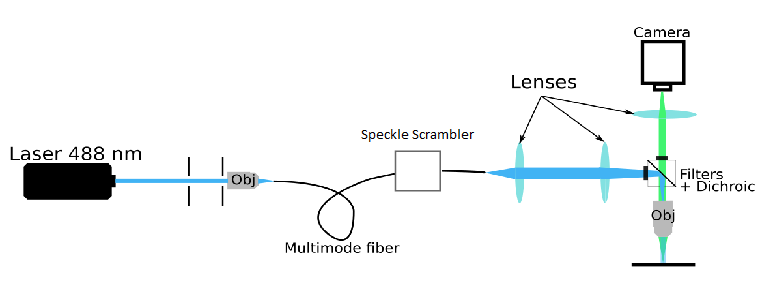
\includegraphics[scale=0.65]{fig/Microtempo.png}
    \caption{Schéma simplifié du microscope HiLo (il ne contient pas la seconde fibre et le module de contrôle de puissance). Le faisceau traverse deux iris avant d'être focalisé à l'entrée d'une fibre multimode par un objectif . Le faisceau est alors imagé sur l'ouverture arrière d'un autre objectif (\textit{Obj}) à l'aide d'un système de deux lentilles (f$_{1} = 100$~mm, f$_{2} = 200$~mm).}
    \label{Fig:Microscope}
\end{figure}

\subsection{Sortie du laser et alignement}

La source d'illumination utilisée pour ce microscope est une diode laser fabriquée par JDSU (P/N: 21075556, S/N: FCD000401). La longueur d'onde de cette diode est de 488~nm. Le faisceau, à la sortie de la diode, est réfléchi sur un miroir, puis passe dans deux iris assez espacés. Le but de placer deux iris est de rendre l'ajout d'autres sources laser simple et facile à réaliser. En effet, si un faisceau qui passe par ces deux iris est aligné avec le reste du montage, alors, si on ajoute une nouvelle source, il suffit de faire passer son faisceau par les deux iris. Par la suite, le faisceau est réfléchi par un nouveau miroir et est envoyé dans le module de contrôle de puissance.

\begin{figure}[h]
    \centering
    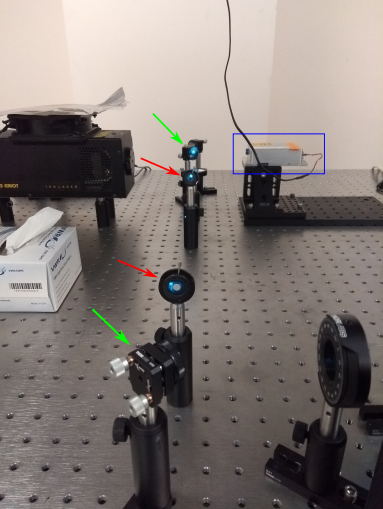
\includegraphics[scale=0.75]{fig/SortieMod.PNG}
    \caption{Image de la diode laser (encadré bleu) et du faisceau qui frappe un miroir (flèche verte du haut), traverse deux iris (flèches rouges) puis frappe un autre miroir (flèche verte du bas) pour se diriger vers le module de contrôle de puissance.}
    \label{Fig:SortieLaser}
\end{figure}

\subsection{Contrôle de la puissance}

Le module de contrôle de puissance est simple: il n'est composé que d'une lame demi-onde (Thorlabs, 400-800~nm) et d'un cube séparateur de polarisation (Thorlabs CM05-PBS201, 420-680~nm) tel qu'illustré sur la figure \ref{Fig:ContPuiss}. Puisque le faisceau est polarisé linéairement à la sortie de la diode, il est possible de modifier l'orientation de cette polarisation à l'entrée du cube en tournant la lame demi-onde. En tournant celle-ci, on modifie la puissance aux deux sorties du cube. En envoyant une sortie dans un piège à faisceau (\textit{beam dump}) et en utilisant l'autre comme illumination pour le reste du montage, on obtient un faisceau dont la puissance est facilement modifiable. À la sortie du cube, le faisceau est prêt à être injecté dans la fibre optique.

\begin{figure}[H]
    \centering
    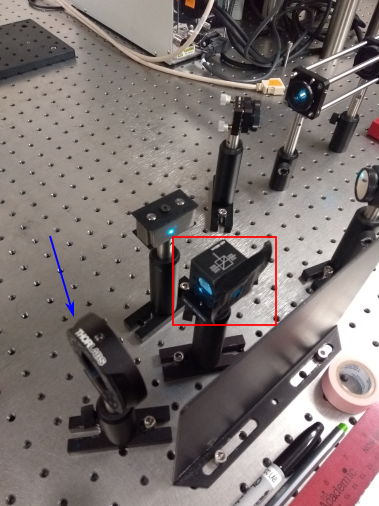
\includegraphics[scale=0.75]{fig/ControlePuissanceMod.PNG}
    \caption{Image du module de contrôle de puissance composé d'une lame demi-onde sur un support rotatif (flèche bleue) et d'un cube séparateur de polarisation (encadré rouge).}
    \label{Fig:ContPuiss}
\end{figure}

\subsection{Injection dans la fibre multimode}

Avant d'être injecté dans la fibre optique multimode, le faisceau est réfléchi sur deux miroirs afin de pouvoir aisément modifier sa position et son angle à l'entrée de la fibre. Toutefois, avant ceci, le faisceau passe par deux iris afin de s'assurer que celui-ci est parallèle à l'axe optique de la fibre. Enfin, la fibre est placée sur un support de translation au plan focal d'un objectif (Olympus 10X, NA~=~0,25).

\begin{figure}[H]
    \centering
    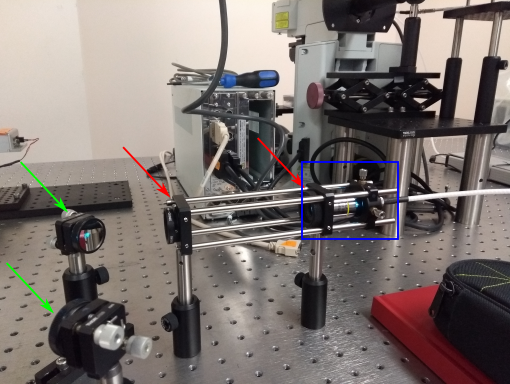
\includegraphics[scale=0.75]{fig/InjectionMod.PNG}
    \caption{Image du trajet du faisceau pour l'injection dans la fibre multimode. Celui-ci frappe deux miroirs (flèches vertes), puis traverse deux iris (flèches rouges) pour finalement converger vers l'entrée d'une fibre optique à l'aide d'un objectif 10X Olympus (encadré bleu).}
    \label{Fig:Inject}
\end{figure}

\subsection{Contrôle de l'illumination (speckles/uniforme)}

Afin de contrôler le mode d'illumination, un \textit{speckle scrambler} (High speed speckle scrambler, S/N: 20172112-4, GigaConcept) est utilisé. Celui-ci est connecté à un module d'acquisition (Labjack U3-HV) afin de communiquer avec l'ordinateur. Toutefois, au moment de la rédaction de ce rapport (3 septembre 2018), le \textit{speckle scrambler} est défectueux et la communication avec le Labjack est impossible. La sortie du \textit{speckle scrambler} est ensuite connectée à une autre fibre optique (Coeur de 1500~$\mu$m, NA~=~0,5, modèle M107L01, Thorlabs). Le but d'ajouter cette fibre avec un plus gros coeur est d'augmenter le nombre de speckles à la sortie de la fibre, ce nombre étant calculé de la façon suivante \cite{FiberStats}:

\begin{equation*}
    N = \pi\left(\frac{2a(\text{NA})}{\lambda}\right)^2
\end{equation*}

où $a$ est le rayon du coeur de la fibre, NA est son ouverture numérique et $\lambda$ est la longueur d'onde du laser. Un support a également été ajouté (figure \ref{Fig:Scrambler}) afin de stabiliser la fibre lors du changement de mode d'illumination.

\begin{figure}[H]
    \centering
    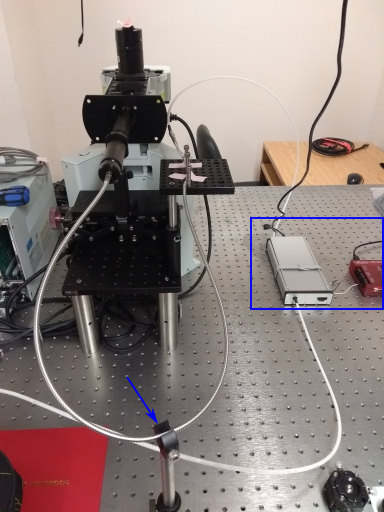
\includegraphics[scale=0.75]{fig/SpeckleScrambler.PNG}
    \caption{Image de la fibre optique et du \textit{speckle scrambler} (encadré bleu). On y voit également le support ajouté (flèche bleue).}
    \label{Fig:Scrambler}
\end{figure}

\subsection{De la sortie de la fibre à l'échantillon}

Le premier problème rencontré à la sortie de la fibre est le fait que l'illumination est très peu uniforme. Puisque tous les modes de la fibre ne sont pas également excités, la sortie peut être très aléatoire. Une façon simple d'uniformiser la sortie est d'appliquer une légère tension dans la fibre, ce qui réorganise les modes excités. Pour ce microscope, la tension est appliqué en faisant passer la fibre entre 3 vis (figure \ref{Fig:Vis}). Ainsi, par essai et erreur, il est possible d'obtenir une illumination beaucoup plus uniforme (figure \ref{Fig:Illumination}).

\begin{figure}[H]
    \centering
    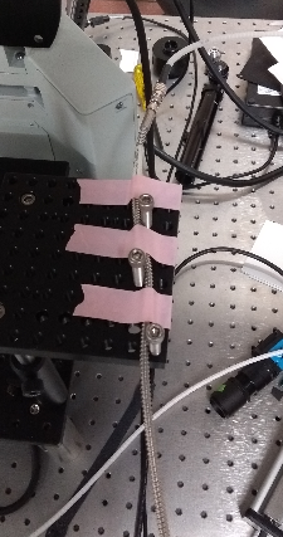
\includegraphics[scale=0.75]{fig/Vis.png}
    \caption{Arrangement de vis pour contrôler la tension appliquée sur la fibre.}
    \label{Fig:Vis}
\end{figure}

\begin{figure}[H]
    \centering
    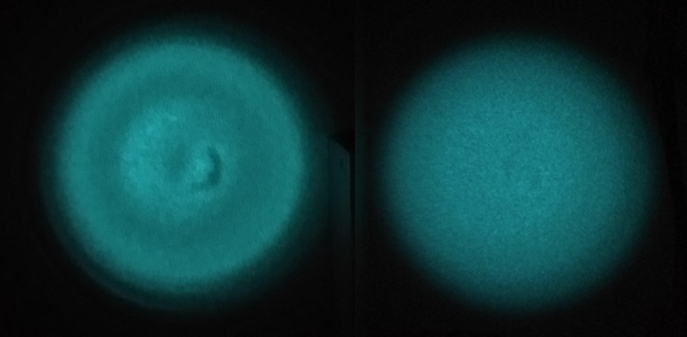
\includegraphics[scale=0.75]{fig/Illumination.png}
    \caption{Différence entre l'illumination sans tension dans la fibre (gauche) et avec tension dans la fibre (droite).}
    \label{Fig:Illumination}
\end{figure}


La sortie de la fibre est fixée à un tube dans lequel se trouve un système 4F de deux lentilles. Ce tube est centré dans une base de microscope (Olympus BX61WI) à l'aide de supports fabriqués sur mesure (la figure \ref{Fig:Support} montre l'allure de ces supports). La fibre se trouve au plan focal de la première lentille (f~=~100~mm) qui est à 300~mm de la seconde (f~=~200~mm). Les lentilles ont été choisies afin d'avoir le plus petit grandissement possible. De cette façon, puisque le faisceau est focalisé sur l'ouverture arrière de l'objectif, la taille du faisceau au point focal de l'objectif est plus grande, ce qui donne un meilleur champ de vue. Le bout de la fibre est imagé sur l'ouverture arrière de l'objectif plutôt que sur l'échantillon justement pour cette raison. Toutefois, avant d'atteindre l'objectif, le faisceau traverse un filtre d'excitation (filtre passe-bande 490/20~nm) et est réfléchi par un miroir dichroïque (Brightline 500~nm edge dichroic mirror, FF500-Di01-25x36).

\begin{figure}[H]
    \centering
    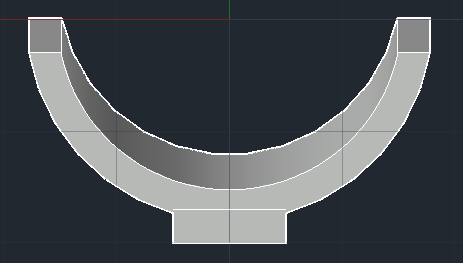
\includegraphics[scale=0.75]{fig/Support.PNG}
    \caption{Dessin d'un des supports utilisés pour centrer le tube contenant les lentilles dans la base de microscope Olympus BX61WI.}
    \label{Fig:Support}
\end{figure}


\subsection{Déplacement de l'échantillon}

La base de microscope Olympus BX61WI est munie d'un moteur permettant le déplacement en Z de l'objectif, ce qui permet d'imager tout le volume des échantillons. Toutefois, elle n'offre pas de déplacement dans le plan horizontal. Pour ceci, une monture motorisée (T-LSM050A, Zaber) est utilisée. Les déplacements peuvent être effectués à l'aide du T-JOY3 de Zaber ou encore par ordinateur pour des déplacements plus précis. Si la monture est connectée à l'ordinateur, il est important que le fil connecté à celui-ci soit connecté à la prise mâle de la monture.

\begin{figure}[H]
    \centering
    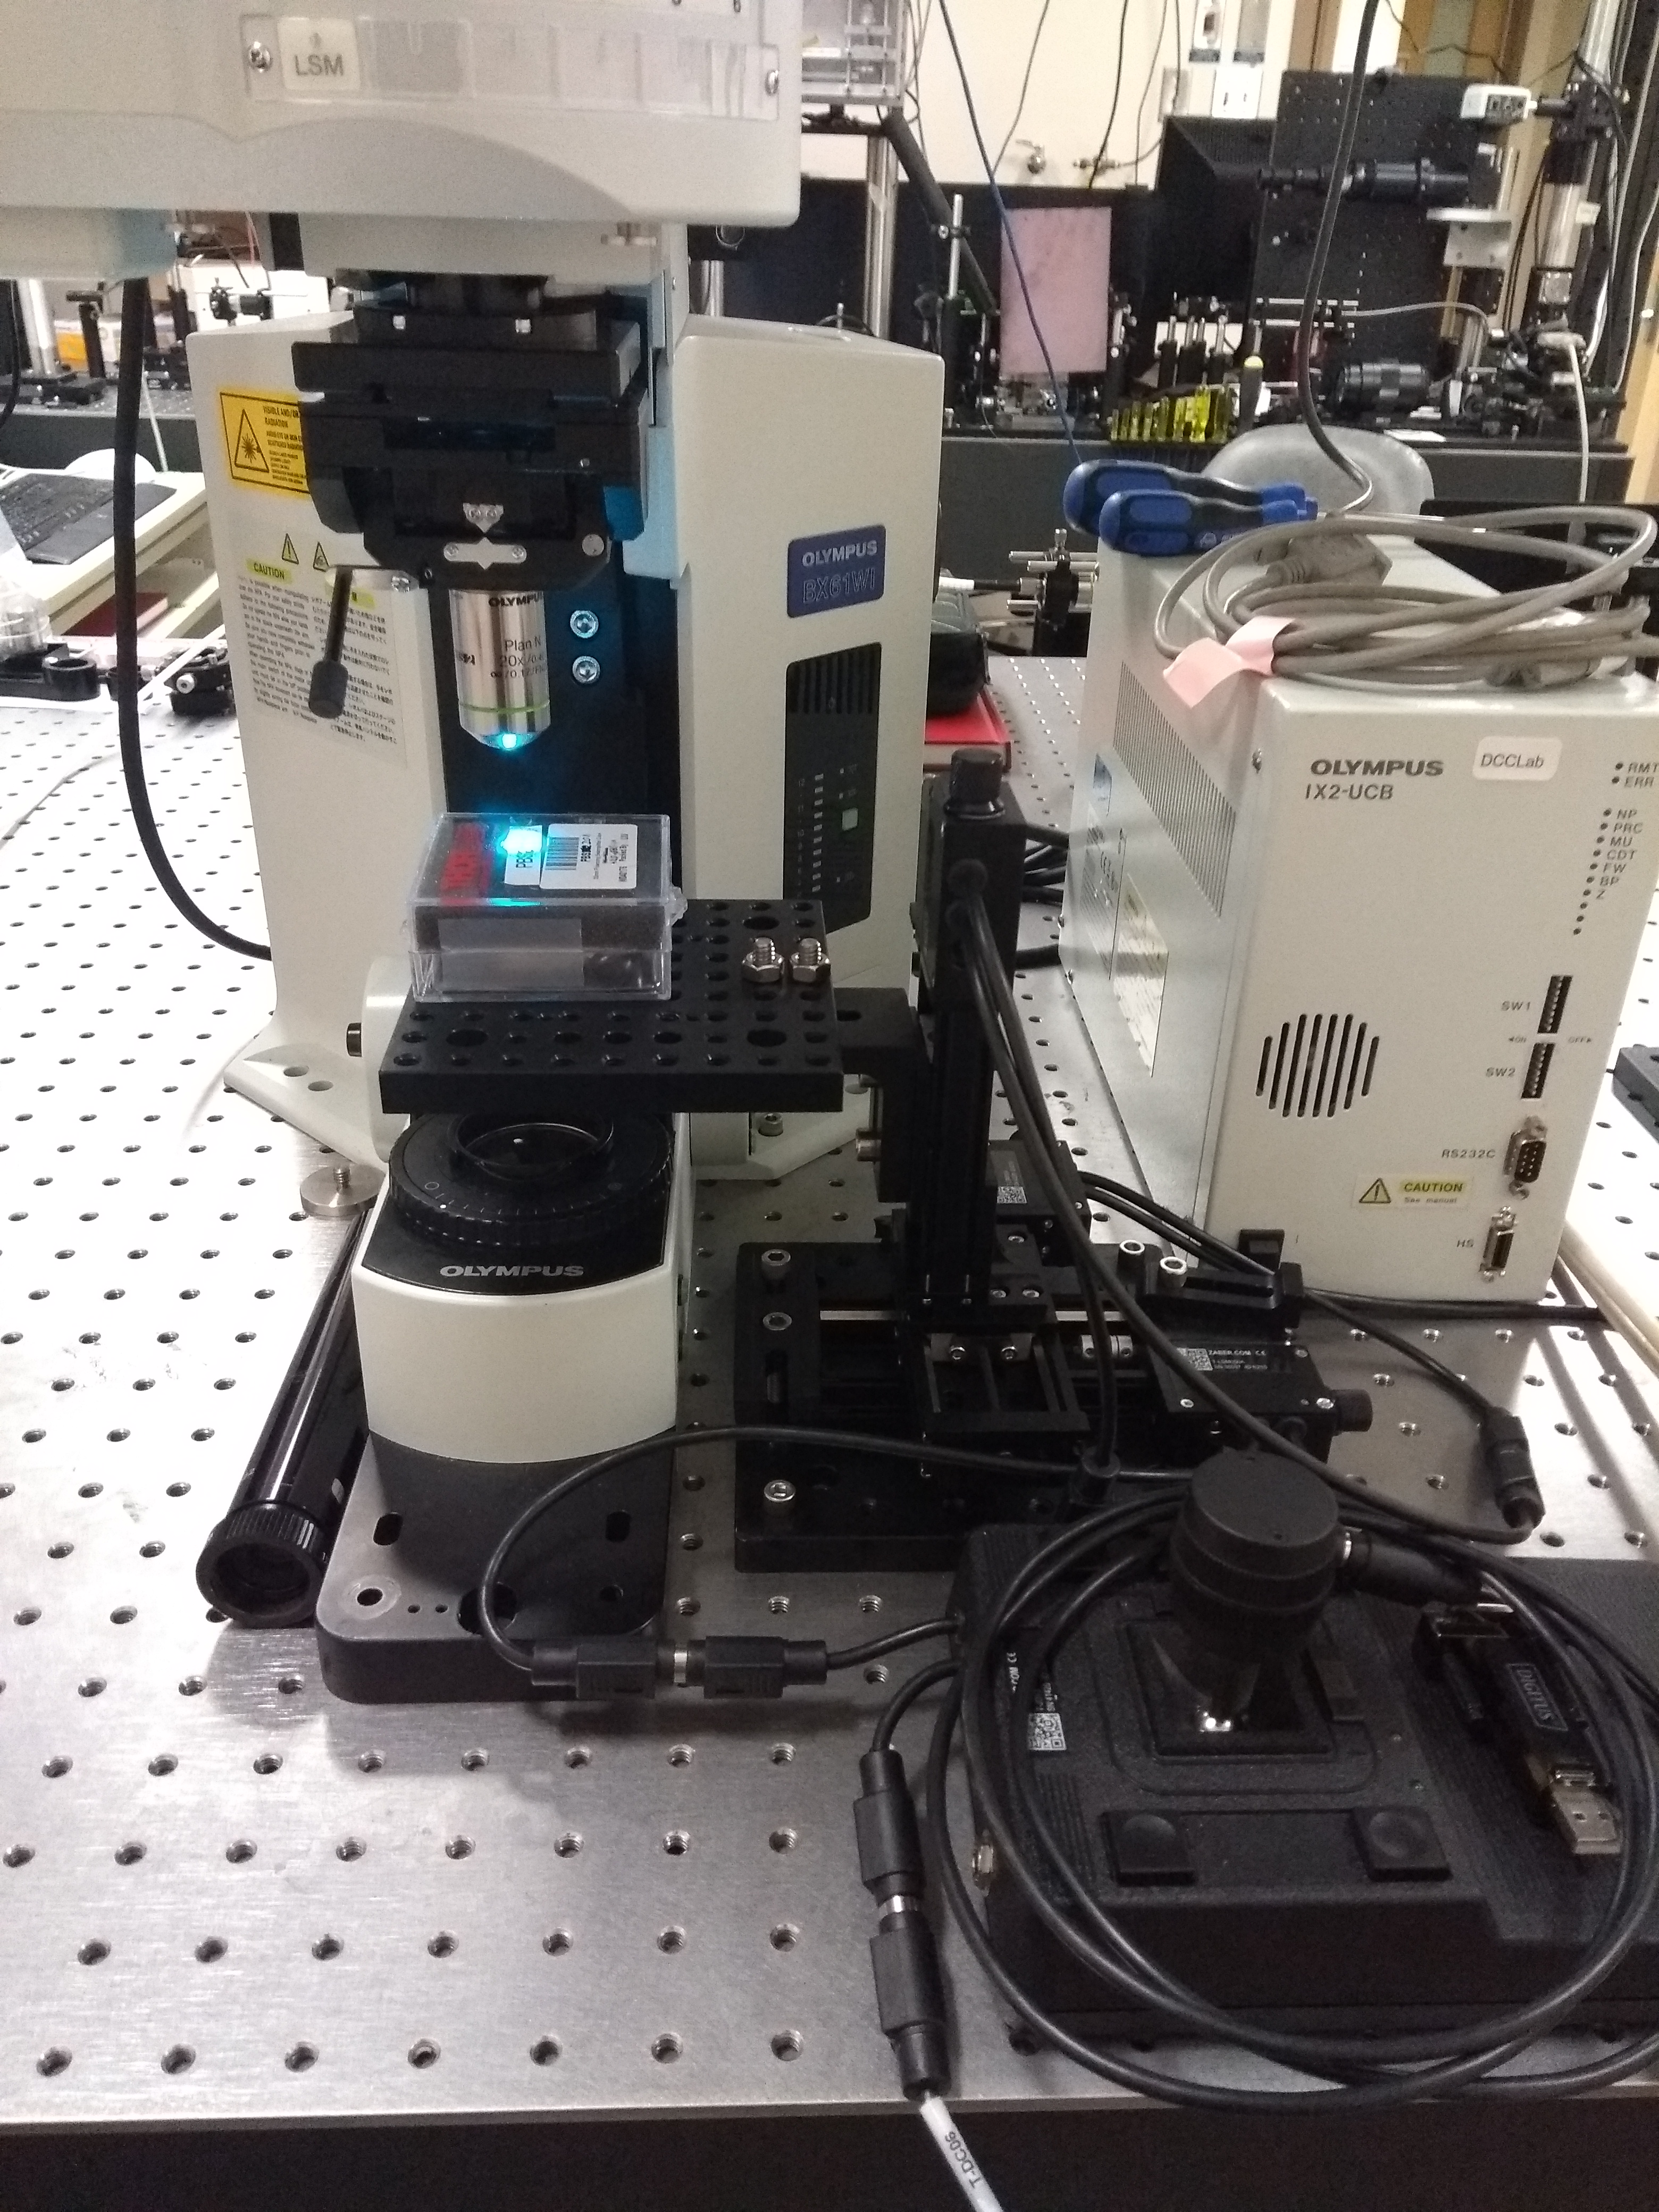
\includegraphics[scale=0.07]{fig/Zaber.jpg}
    \caption{Image de la sortie de l'objectif sur l'échantillon ainsi que de la base motorisée Zaber.}
    \label{Fig:Zaber}
\end{figure}

\subsection{Récupération de la fluorescence}

Enfin, afin de récupérer la fluorescence émise par l'échantillon, le faisceau traverse le miroir dichroïque ainsi qu'un filtre d'émission (filtre passe-haut FF01-496/LP-25, Brightline), puis l'échantillon est imagé sur le capteur CCD d'une caméra à l'aide d'un coupleur (Olympus U-TV0.5XC-3). La caméra utilisée est la Orca Flash 4.0 de Himamatsu et est connectée à l'ordinateur via une carte d'acquisition (carte Active Silicon dans une boîte Sonnet).



\section{Les résultats}
\label{Results}

À la fin de l'été, le stagiaire commençait à tester la prise d'images avec le microscope. Pour cette raison, peu de résultats sont disponibles. Toutefois, une acquisition de deux grains de pollen côte-à-côte a été effectuée. Un des plans de l'acquisition est illustré à la figure \ref{Fig:Grains}. Les grains de pollen ont un diamètre approximatif de 25 $\mu$m et un objectif 40X est utilisé pour l'imagerie. D'autres acquisitions, notamment de billes fluorescentes et d'une lame fluorescente, sont disponibles sur le serveur Cafeine2 de DCC-Lab dans le dossier dcc-lab. Un problème soulevé lors de cette acquisition est que le sectionnement optique ne semble pas être optimal. En effet, lorsque le grain de pollen s'éloigne du plan focal, plutôt que de le voir disparaître, on obtient plutôt un étalement de la fluorescence (voir la figure \ref{Fig:Etalement}). Ce problème reste à régler.

\begin{figure}[H]
    \centering
    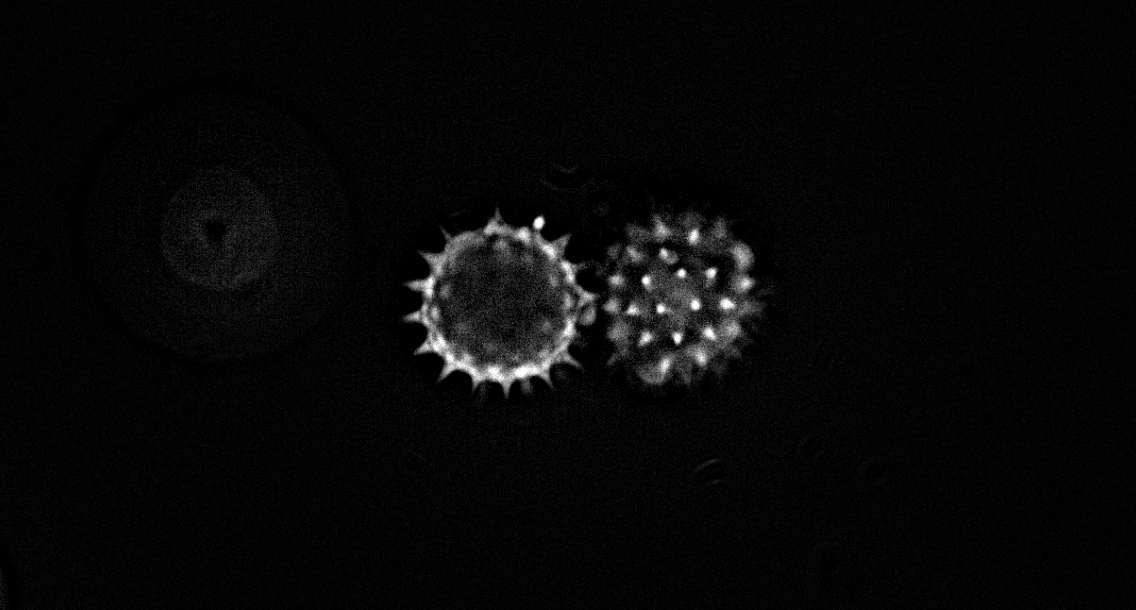
\includegraphics[scale=0.4]{fig/BeauPollen.PNG}
    \caption{Une tranche d'une acquisition sur tout le volume de deux grains de pollen après sectionnement optique par traitement HiLo. Cette image est un agrandissement de l'image obtenue lors de l'acquisition.}
    \label{Fig:Grains}
\end{figure}

\begin{figure}[H]
    \centering
    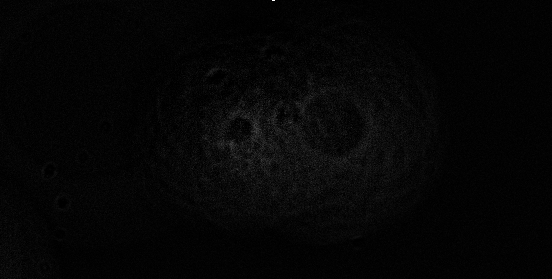
\includegraphics[scale=0.8]{fig/Etalement.PNG}
    \caption{Autre tranche de l'acquisition des deux grains de pollen. Cette tranche est à 30~$\mu$m de celle illustrée à la figure \ref{Fig:Grains}. Bien que les grains ne devraient plus être au plan focal, on remarque tout de même un espèce d'étalement de la lumière recueillie. Cette image est un agrandissement de l'image obtenue lors de l'acquisition.}
    \label{Fig:Etalement}
\end{figure}

\section{La suite}

En somme, un prototype fonctionnel de microscope HiLo a été assemblé. Toutefois, le travail n'est pas terminé. En effet, il serait intéressant de faire d'autres acquisitions, notamment de poissons zèbre afin de voir si le sectionnement optique est propice à l'imagerie de neurones. Il reste également à quantifier les performances du microscope ainsi qu'à tenter de régler le problème de sectionnement énoncé à la section \ref{Results}.




\newpage


\begin{thebibliography}{9}

\bibitem{Manuel} Goodman, Joseph W., \emph{Speckle phenomena in optics: theory and applications}, Roberts and Company Publishers (2007), page 18

\bibitem{Mertz2008} Lim, D., Chu, K. K. et Mertz, J. \emph{Wide-field fluorescence sectioning with hybrid
speckle and uniform-illumination microscopy}, Optics Letters, Vol. 33 No. 16 (2008).

\bibitem{Mertz2011} Lim, D. et al. \emph{Optically sectioned in vivo imaging with speckle
illumination HiLo microscopy}, Journal of Biomedical Optics (2011).

\bibitem{FiberStats} Masaaki, Imai, \emph{Statistical Properties of Optical Fiber Speckles}, Bulletin of the Faculty of Engineering, Hokkaido University (1985)


\bibitem{Wiki} Wikipedia, \emph{Tavelures (optique)}, En ligne, \url{https://fr.wikipedia.org/wiki/Tavelure_(optique)}


\end{thebibliography}

\end{document}